% A0 portrait poster: flat cobalt illustrations on cream, chunky rounded type.
% Compile with LuaLaTeX, twice:  lualatex poster-brand.tex
% Illustrations: put traced SVG->PDF (or PNG) files in illustrations/ with the names used below;
% until a file exists, a dashed placeholder shows where it goes.
\documentclass{article}
\usepackage[paperwidth=841mm,paperheight=1189mm,margin=6.5cm,top=5.5cm,bottom=5cm]{geometry}
\usepackage{fontspec}
\usepackage{xcolor,graphicx,tikz}
\pagestyle{empty}
\setlength{\parindent}{0pt}

% ---- Fonts ----
\newfontfamily\chunky{Sniglet-ExtraBold.ttf}[Path=fonts/]
\newfontfamily\soft{Sniglet-Regular.ttf}[Path=fonts/]
\setmainfont{Seravek}[BoldFont={Seravek Medium}]

% ---- Colours ----
\definecolor{cream}{HTML}{FBF7EE}
\definecolor{cobalt}{HTML}{1F3FBF}
\definecolor{ink}{HTML}{1B1F3B}
\definecolor{soft}{HTML}{6A6F8C}
\pagecolor{cream}
\color{ink}

\newcommand{\body}{\fontsize{34}{47}\selectfont}

% \illus{file name without extension}{height}{what goes here}
\newcommand{\illus}[3]{%
  \IfFileExists{illustrations/#1.pdf}{\includegraphics[height=#2]{illustrations/#1.pdf}}{%
  \IfFileExists{illustrations/#1.png}{\includegraphics[height=#2]{illustrations/#1.png}}{%
  \tikz\node[draw=cobalt!40, dashed, line width=2.5pt, rounded corners=12mm, minimum height=#2,
    minimum width=#2, align=center, text=cobalt!60, font=\soft\fontsize{30}{38}\selectfont]{#3\\[4mm]\fontsize{22}{26}\selectfont\ttfamily #1};}}}

% Section: big chunky title, then body
\renewcommand{\section}[1]{{\chunky\color{cobalt}\fontsize{66}{70}\selectfont #1\par}\vspace{8mm}}

% Big number with a label underneath: \stat{44.81}{overall, ours}
\newcommand{\stat}[2]{\begin{minipage}[t]{0.3\linewidth}\centering
  {\chunky\color{cobalt}\fontsize{104}{104}\selectfont #1\par}\vspace{4mm}{\soft\fontsize{32}{38}\selectfont #2\par}\end{minipage}}

\begin{document}

% =================== TOP: logo, title, QR ===================
\begin{minipage}[c]{0.2\linewidth}
  
\includegraphics[width=\linewidth]{bocconi-logo-cobalt.pdf}
\end{minipage}\hfill
\begin{minipage}[c]{0.14\linewidth}\raggedleft
  
\includegraphics[width=0.85\linewidth]{repo-qr-cobalt.png}\par\vspace{2mm}
  {\soft\color{soft}\fontsize{24}{28}\selectfont code on github}
\end{minipage}

\vspace{6mm}
\begin{minipage}[c]{0.6\linewidth}
  {\raggedright\chunky\color{cobalt}\fontsize{120}{124}\selectfont what a camera's\\ path knows\\ about activity\par}
  \vspace{16mm}
  {\fontsize{40}{50}\selectfont Juan Ignacio Arguello \,·\, Valerio Costa \,·\, Facundo Lucero\par}
  \vspace{4mm}
  {\color{soft}\fontsize{28}{36}\selectfont 20600 Deep Learning for Computer Vision \,·\, Bocconi University \,·\, Prof.~Chiara Plizzari\par}
\end{minipage}\hfill
\begin{minipage}[c]{0.36\linewidth}\centering
  \illus{hero}{21cm}{hero: person with a\\camera on their head}
\end{minipage}

\vspace{16mm}
% =================== THE QUESTION: cobalt band ===================
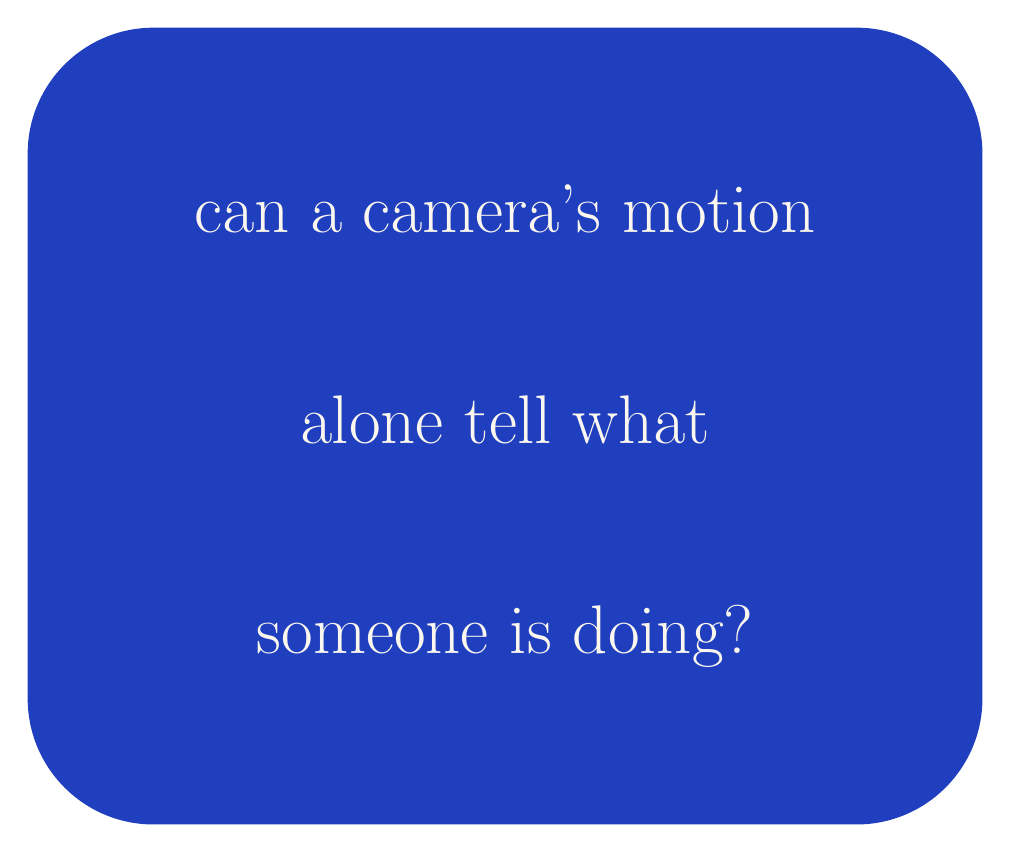
\begin{tikzpicture}
  \node[fill=cobalt, rounded corners=16mm, text width=\linewidth-40mm, inner sep=20mm, align=center,
    text=cream, font=\chunky\fontsize{66}{76}\selectfont]
    {can a camera's motion alone tell what someone is doing?};
\end{tikzpicture}

\vspace{16mm}
% =================== PROBLEM + METHOD ===================
\begin{minipage}[t]{0.47\linewidth}
  \section{the problem}
  {\body [Two or three short lines: egocentric video, why poses only, what CamFormer does.]\par}
  \vspace{10mm}
  {\centering\illus{path}{12cm}{a camera path\\swirling through a room}\par}
\end{minipage}\hfill
\begin{minipage}[t]{0.47\linewidth}
  \section{how it works}
  {\body [One or two lines: poses into CamFormer, text into a text encoder, matched with a contrastive loss.]\par}
  \vspace{10mm}
  {\centering\illus{method}{12cm}{pipeline: path $\rightarrow$ model\\$\leftrightarrow$ words}\par}
\end{minipage}

\vspace{16mm}
% =================== REPRODUCTION: big numbers ===================
\section{we reproduced it}
\stat{[x]}{overall, paper}\hfill\stat{44.81}{overall, ours}\hfill\stat{33.61}{procedural, ours}

\vspace{16mm}
% =================== THREE EXTENSIONS ===================
\section{then we tried three things}
\vspace{6mm}
\begin{minipage}[t]{0.3\linewidth}\centering
  \illus{negatives}{9cm}{hard negatives}\par\vspace{8mm}
  {\chunky\color{cobalt}\fontsize{48}{54}\selectfont hard negatives\par}\vspace{4mm}
  {\body [one line + one number]\par}
\end{minipage}\hfill
\begin{minipage}[t]{0.3\linewidth}\centering
  \illus{egoexo}{9cm}{one model,\\two views}\par\vspace{8mm}
  {\chunky\color{cobalt}\fontsize{48}{54}\selectfont one ego + exo model\par}\vspace{4mm}
  {\body [one line + one number]\par}
\end{minipage}\hfill
\begin{minipage}[t]{0.3\linewidth}\centering
  \illus{eye}{9cm}{an eye}\par\vspace{8mm}
  {\chunky\color{cobalt}\fontsize{48}{54}\selectfont eye gaze\par}\vspace{4mm}
  {\body [one line + one number]\par}
\end{minipage}

\vspace{14mm}
% =================== TAKEAWAYS ===================
\section{what we learned}
{\body
\textcolor{cobalt}{\chunky 1}\quad [First finding, one line.]\par\vspace{6mm}
\textcolor{cobalt}{\chunky 2}\quad [Second finding, one line.]\par\vspace{6mm}
\textcolor{cobalt}{\chunky 3}\quad [Third finding, one line.]\par}

\vfill
{\centering\soft\color{soft}\fontsize{26}{32}\selectfont after \emph{seeing without pixels} (camformer) \,·\, data: ego-exo4d\par}
\end{document}
